\documentclass[xcolor={rgb}]{beamer}
\usepackage[labelformat=empty]{caption}

\newcommand{\pitem}{\pause\item}
\usetheme{metropolis}

\author{Alireza Arzehgar}
\title{Introduction to Distributed Systems}
\date{\today}

\begin{document}
	% Talk about presentation approachs.
	% I wanna handle it very interactive. Audience should help me to asking questions
	% and answering them.
	\begin{frame}[plain]
		\titlepage
	\end{frame}

	% Explain about what is system, components and their dependencies.
	% Then open up distributed systems and talk about independent components.
	\begin{frame}[plain,c]
		\begin{center}
		\Huge What are Systems and Distributed Systems?
		\end{center}
	\end{frame}

	% Talk about requirements. Is your system resource usage or data volume will
	% increase 100 times in the future? What is your current needs?
	% Are you care about 5 hours down time due server outage or disk failure?
	% Have you high traffic and performance target or multi geographic users?
	% Based on your answers we should choose system architecture
	\begin{frame}{Non-Functional System Requirements}
	\begin{itemize}
		\pitem Reliability
		\pitem Performance
		\pitem Scalability
	\end{itemize}
	\end{frame}

	% First of all I talk about scalability.
	% Explain two system scaling architecture and flash-back to previous talks.
	% Your architecture choice will be dependent on your requirements.
	\begin{frame}{Scaling to Higher Load}
		\begin{itemize}
			\pitem Vertical Scaling \\
				\pause \textbf{Architecture}: Shared-Memory \\
				\pause \textbf{Drawback}:$ Cost(2R) > 2Cost(R) $ \\
				$ Performance(2x) < 2Performance(x) $
			\pitem Horizontal Scaling \\
				\pause \textbf{Architecture}: Shared-Nothing \\
				\pause \textbf{Drawback}: Additional Complexity \& Operational Overhead
		\end{itemize}
	\end{frame}

	% How we can scale following resources in high load?
	% Ask to audience for guessing scaling solution for storage read load
	% using distributed systems.
	\begin{frame}{Scalability - Problems}
	\begin{itemize}
		\pitem CPU \& Memory Usage
		\pitem Storage Read Load
		\pitem Storage Data Volume
		\pitem Storage Write Load
	\end{itemize}
	\end{frame}

	% Talk about Amdahl's Law, simple example of when Shared-Memory Architer
	% doesn't scale well.
	\begin{frame}{Scalability - Problems}
		\begin{center}
		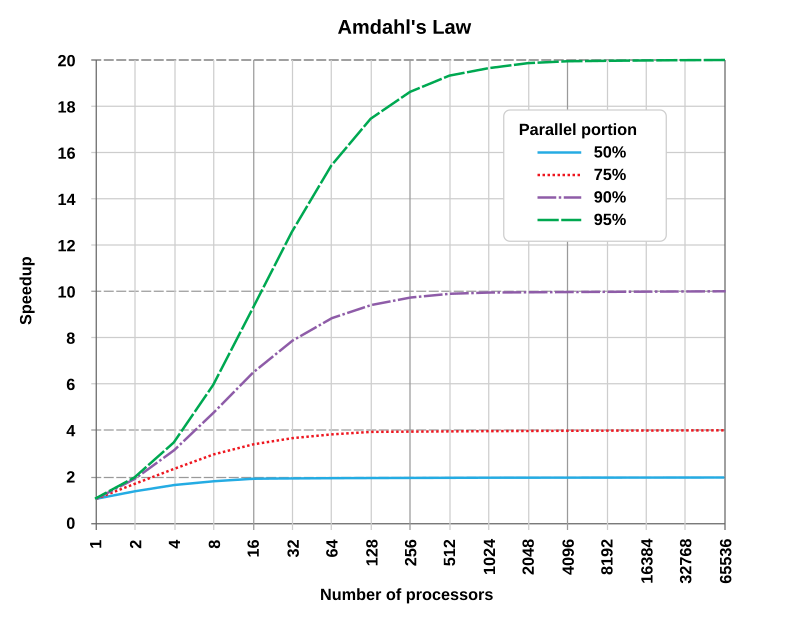
\includegraphics[width=\textwidth]{assets/amdahl.png}
		\end{center}
	\end{frame}

	% Talk about other scenarios and let audience guess
	% How to solve them using offered solutions
	\begin{frame}{Reliability and Performance - Problems}
	\begin{itemize}
		\pitem \textbf{Reliability}: System Faults
		\begin{itemize}
			\pitem Server Outages
			\pitem Network Problems
			\pitem Datacenter Outages
		\end{itemize}
		\pitem \textbf{Performance}: Latency
	\end{itemize}
	\end{frame}

	% LoadBalancing in stateless applications and combining with other solutions (Replication)
	% It will help to scale CPU & Memory Usage, Storage Load and even Reliability and Latency problems
	\begin{frame}{Load Balancing}
		\begin{center}
		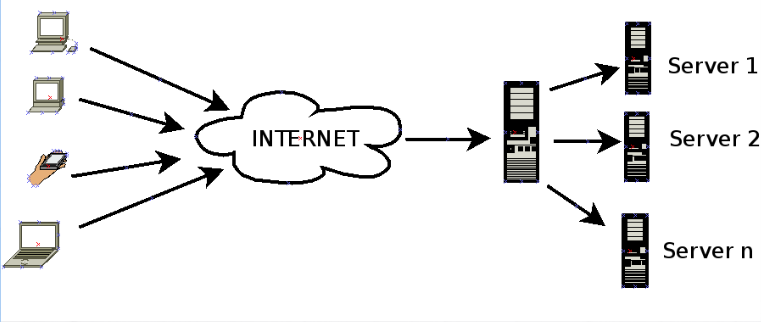
\includegraphics[width=\textwidth]{assets/loadbalancer.png}
		\end{center}
	\end{frame}

	% Keep and sync copy of data/workload to multiple machines.
	% It will help to read load and also System Usage
	% Ask for more replication methods
	\begin{frame}{Replication}
		\begin{center}
		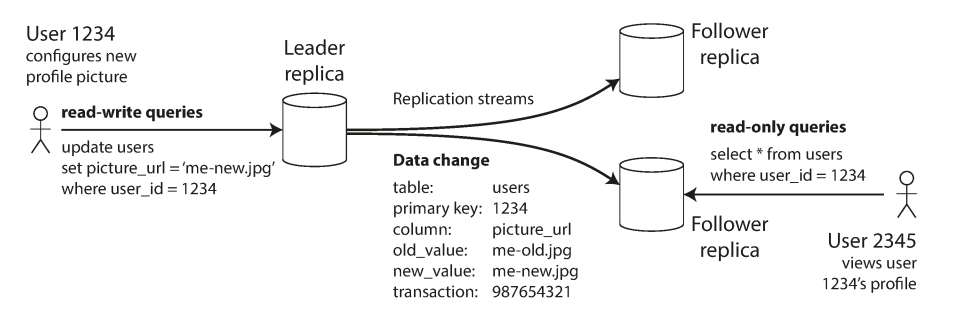
\includegraphics[width=\textwidth]{assets/replication.png}
		\end{center}
	\end{frame}

	% Split data to multiple mahcines (this is simplest sharding algorithm. sharding by key range)
	% This strategy will scale data volume and write load
	% Ask for more sharding algorithms
	\begin{frame}{Sharding}
		\begin{center}
		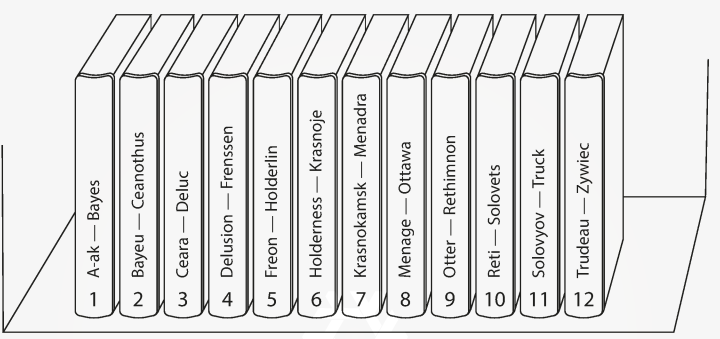
\includegraphics[width=\textwidth]{assets/sharding.png}
		\end{center}
	\end{frame}

	% Summary for scalability problems and solutions
	\begin{frame}{Scalability - Problems vs Solutions}
	\begin{itemize}
		\pitem Problems
		\begin{itemize}
			\item CPU \& Memory Usage
			\item Storage Read Load
			\item Storage Data Volume
			\item Storage Write Load
		\end{itemize}

		\pitem Solutions
		\begin{itemize}
			\item Load Balancing
			\item Replication
			\item Sharding
		\end{itemize}
	\end{itemize}
	\end{frame}

	% How load balancer in stateless applications and replication in stateful
	% applications will help to Reliability and Performance
	\begin{frame}{Reliability and Performance - Solutions}
	\begin{center}
		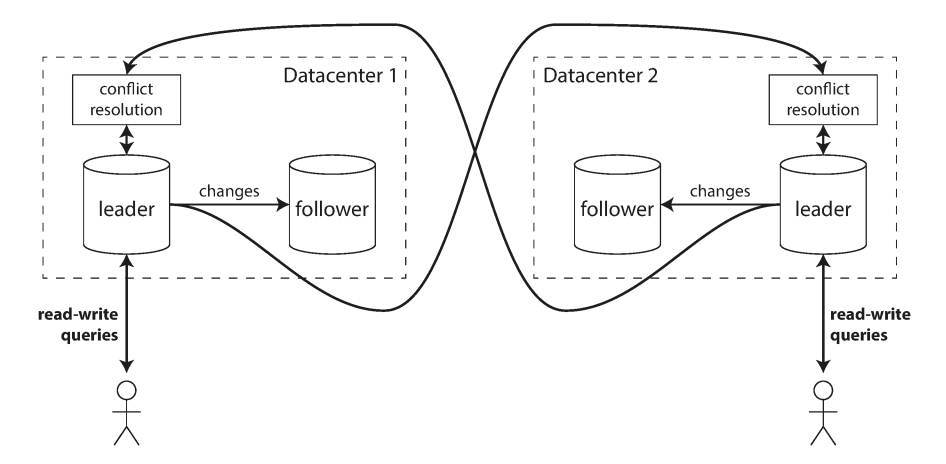
\includegraphics[width=0.9\textwidth]{assets/multileader.png}
	\end{center}

	\begin{itemize}
		\pitem \textbf{Reliability}: System Faults
		\begin{itemize}
			\pitem Server Outages
			\pitem Network Problems
			\pitem Datacenter Outages
		\end{itemize}
		\pitem \textbf{Performance}: Latency
	\end{itemize}
	\end{frame}

	% Talk about distributed systems drawbacks and nothing is god
	\begin{frame}[plain,c]
		\begin{center}
		\Huge There is no such thing as a generic, one-size-fits-all scalable architecture.
		\end{center}
	\end{frame}

	% Discussion
	\begin{frame}[plain,c]
		\begin{center}
		\Huge Q\&A
		\end{center}
	\end{frame}
\end{document}
